\documentclass[10pt]{article}
% \usepackage[letterpaper,text={6.5in,8.7in},centering]{geometry}
\usepackage{curves}
\usepackage{epic,eepic,color}
%\usepackage[usenames,dvipsnames,svgnames,table]{xcolor}
% \usepackage{amssymb,amsmath,times,subfigure,graphicx,theorem}
\usepackage{alltt}
%\usepackage{warmread}
%\usepackage[all,import]{xy}
%\usepackage{eepic}
\usepackage{my_packages}
\usepackage{tikz_packages}
\renewcommand{\baselinestretch}{1.2}
\date{}

\renewcommand{\thesubsection}{\arabic{subsection}. }
\renewcommand{\thesubsubsection}{\arabic{subsection}.\arabic{subsubsection} }

\theoremstyle{definition}
\newtheorem{prob}{Problem}[section]
%\renewcommand{\theprob}{\arabic{section}.\arabic{prob}}
\renewcommand{\theprob}{\arabic{prob}}

\newenvironment{subprob}%
{\renewcommand{\theenumi}{\alph{enumi}}\renewcommand{\labelenumi}{(\theenumi)}\begin{enumerate}}%
{\end{enumerate}}%


%1: Explain the Newtonian gravitational force and gravitational potential between particles
%2: Analyze the characteristics of circular, elliptic, parabolic and hyperbolic orbits in a two-dimensional plane
%3: Describe the geometry of an orbit in a three-dimensional space from orbital elements
%4: Find an orbital position as a function of time


\begin{document}


\vspace*{1cm}

\pagestyle{empty}
\centerline{\LARGE{ MAE3145: Midterm Exam}}
\vspace*{0.5cm}
\centerline{\Large October 25, 2017}%\\%\vspace*{0.5cm}

\vspace*{6cm}

\centerline{
\begin{tabular}{lll}
\hspace*{5cm}, & \hspace*{5cm}. & \hspace*{4cm}\\\hline
Last Name & First Name & Student ID
\end{tabular}}

\vspace*{6cm}

\centerline{
\begin{tabular}{|c|c|c|c|c|c|}\hline
Prob. 1 & Prob. 2 & Prob. 3 & Prob. 4 & Prob. 5 & Total \\
(15) & (12) & (16) & (16) & (15) & (74)\\ \hline
\hspace*{2.2cm} & \hspace*{2.2cm} & \hspace*{2.2cm} & \hspace*{2.2cm} & \hspace*{2.2cm} & \hspace*{2.6cm} \\
&&&&&\\
&&&&&\\\hline
\end{tabular}}

$ $\clearpage\newpage$ $

\renewcommand{\thepage}{\arabic{page}/7}
\clearpage\newpage\setcounter{page}{1}\pagestyle{plain}

\renewcommand{\theprob}{\arabic{prob} \textit{(15pt)}}
\begin{prob}
Mark whether each statement written in \textit{italic font} is True or False.
\begin{subprob}


%\item \textit{The orbital speed of the Mars around the Sun is greater than that of the Earth.} [True, False]
%
%\vfill
%
%\item Consider the following two spacecraft, namely $A$ and $B$ on circular orbits. 
%The orbital radius and the mass of them are denoted by $r_A,m_A$, and $r_B,m_B$, respectively. Suppose that $r_B=2r_A$ and $m_B=3m_A$. Then, \textit{the gravitational potential energy of Spacecraft $A$ is greater than that of Spacecraft $B$}. [True, False]\\
%(Hint: $U=-\frac{GMm}{r}$)
%
%
%%\vspace*{0.3cm}
%%\centerline{
%%\setlength{\unitlength}{2.5em}\centering\footnotesize
%%\begin{picture}(3,3)(-1.5,-1.5)
%%\put(0,0){\circle*{0.3}}
%%\put(0,0){\circle{1.5}}
%%\put(0,0){\circle{3}}
%%\put(0.6495,0.3750){\circle*{0.1}}
%%\put(1.5,0){\circle*{0.06}}
%%\put(1.6,-0.3){$B$}
%%\put(0.8,0.3){$A$}
%%\put(3,-0.2){\shortstack[c]{$r_B=2r_A$\\$m_B=0.3m_A$}}
%%\end{picture}}
%
%\vfill 
%
%\item For the two spacecraft $A$ and $B$ discussed above at the part (b), \textit{the \underline{specific} orbital energy of Spacecraft $A$ is greater than that of Spacecraft $B$, i.e. $\mathcal{E}_A > \mathcal{E}_B$}. [True, False]
%
%
%\vfill

\item International space station (ISS) is on a circular orbit at the altitude of $422\,\mathrm{km}$, and GPS satellites are on circular orbits at the altitude of $20200\,\mathrm{km}$. \textit{The specific orbital energy of ISS is greater than GPS satellites, i.e. $\mathcal{E}_{ISS} > \mathcal{E}_{GPS}$}, [True, False]

\vspace*{1cm}

\item \textit{The orbital period of ISS is greater than GPS satellites, i.e. $T_{ISS} > T_{GPS}$}, [True, False]

\vspace*{1cm}

%\item Two circular orbits, namely Orbit 1 and Orbit 2 are illustrated with respect to the geocentric equatorial frame as follows, where gray circles denote the Earth equatorial plane, and the blue circle and the green circle denote the orbital plane for Orbit 1 and Orbit 2, respectively. Note that spacecraft on Orbit 1 is rotating \underline{clockwise}, and spacecraft on Orbit 2 is rotating \underline{counterclockwise}. Then, \textit{the longitude of ascending node of Orbit 1 is greater than Orbit 2, i.e. $\Omega_1 > \Omega_2$.} [True, False]
%
%\renewcommand{\thesubfigure}{}
%\setlength{\unitlength}{0.1\textwidth}
%\begin{figure}[h]
%\centerline{\footnotesize
%	\subfigure[Orbit 1]{\begin{picture}(2.2,2.25)(0,0.05)
%	\put(0,0.395){\includegraphics[width=0.25\textwidth]{prob1c1}}
%	\put(0.2,0.4){$\vec X$}
%	\put(2.5,0.6){$\vec Y$}
%	\put(1.25,2.2){$\vec Z$}
%	\end{picture}}\hspace*{0.2\textwidth}
%	\subfigure[Orbit 2]{\begin{picture}(2.2,2.25)(0,0.05)
%	\put(0,0){\includegraphics[width=0.25\textwidth]{prob1c2}}
%	\put(0.2,0.5){$\vec X$}
%	\put(2.4,0.6){$\vec Y$}
%	\put(1.25,2.3){$\vec Z$}
%	\end{picture}}
%}
%\end{figure}


\item The Aitken basin is the largest crater on the far side of the Moon. The following two lunar orbits, namely Orbit 1 and Orbit 2 are proposed to generate a topographic map of the Aitken basin, which is denoted by $A$ below. The size and the shape of two orbits are identical, i.e., $a_1=a_2$, $e_1=e_2$, and $T_1=T_2$. Assume that the Moon is not rotating: $A$ is stationary with respect to both orbits. Then, \textit{spacecraft on Orbit 1 can take images of $A$ for a longer time period per each revolution than another spacecraft on Orbit 2}. [True, False]

\definecolor{dunkelmagenta}{rgb}{.3, 0, .3}


\vspace*{0.3cm}
\centerline{
\setlength{\unitlength}{0.08\textwidth}\centering\footnotesize
\begin{picture}(3,2)(-1.5,-1)
\put(0,0){\circle*{0.4}}
\put(1.0,0){\ellipse{3.0}{2}}
{\filltype{white}
\put(0.2,0.0){\circle*{0.06}}}
\put(0.9,-1.2){\text{Orbit 2}}
\put(0.25,0.05){$A$}
\put(-0.25,-0.4){\text{Moon}}
\put(1.0,-1){\vector(1,0){0}}
\put(1.0,1){\vector(-1,0){0}}
\color{blue}\put(-1.0,0){\ellipse{3.0}{2}}
\put(-1.0,-1){\vector(1,0){0}}
\put(-1.0,1){\vector(-1,0){0}}
\put(-1.6,-1.2){\text{Orbit 1}}
\end{picture}}
%
\vspace*{1cm}

\item Ground track of a satellite is the projection of the orbit of the satellite onto the surface of the Earth. Ground tracks for two satellites are illustrated as follows. \textit{The inclination of Satellite 1 is greater than Satellite 2, i.e. $i_1> i_2$}. [True, False]

\centerline{
\setlength{\unitlength}{0.1\textwidth}\centering
\begin{picture}(6,3.2)(0,0)\footnotesize
\put(0,0){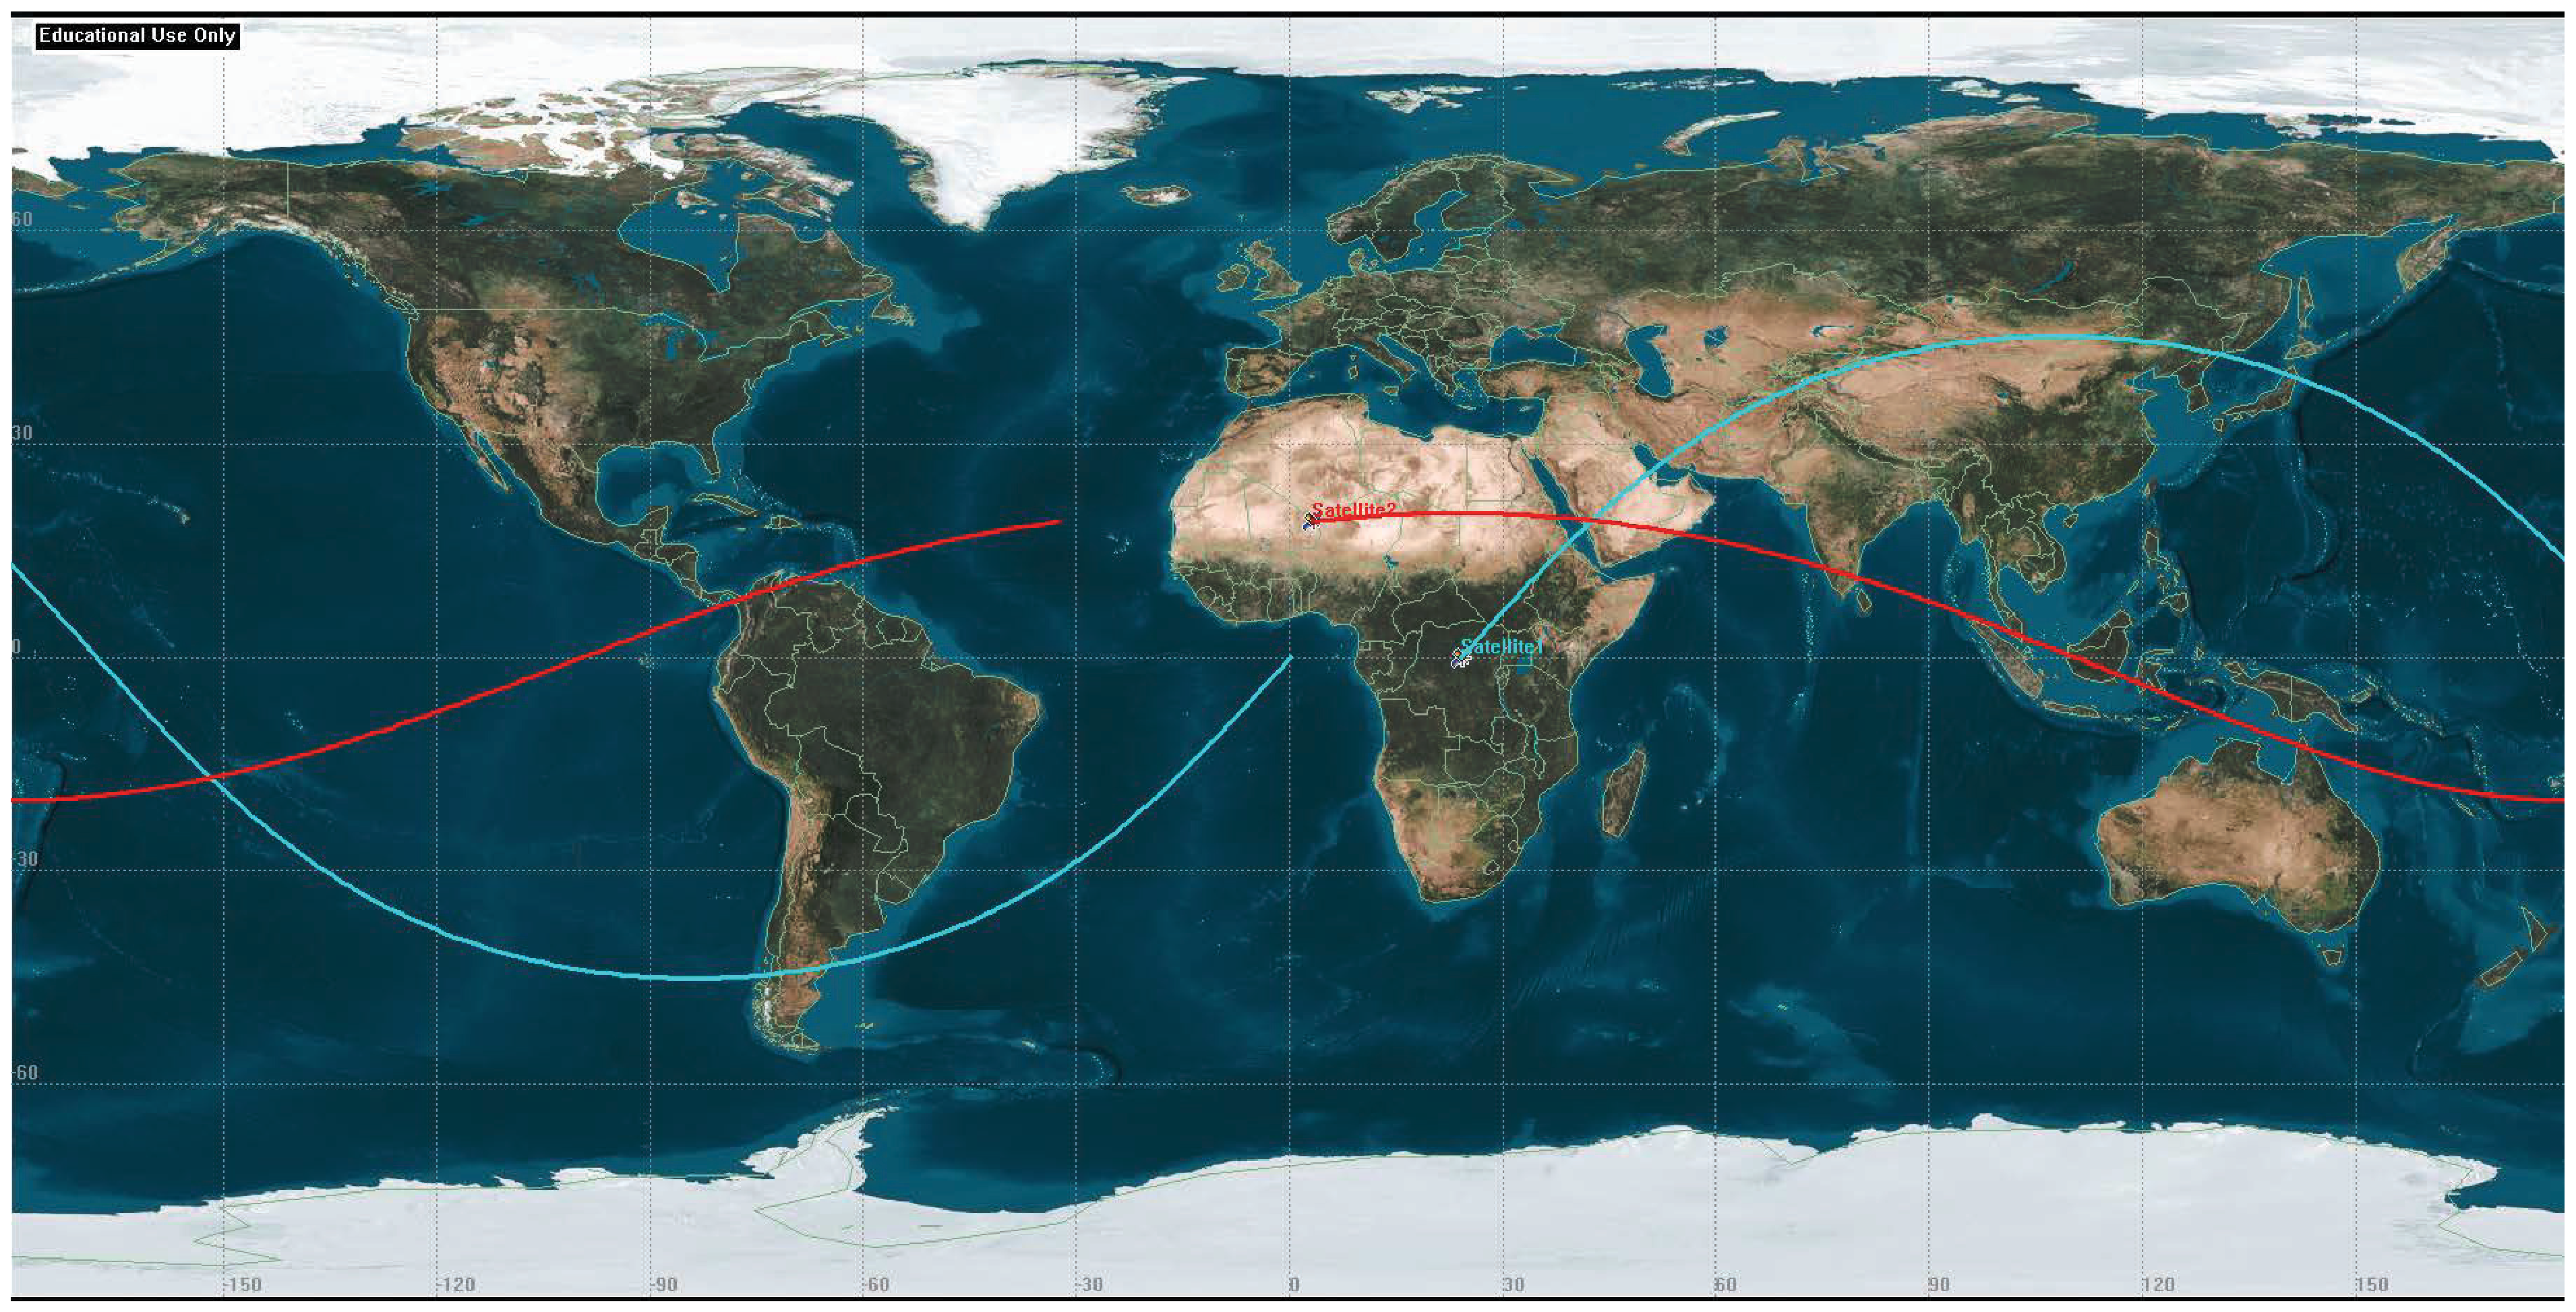
\includegraphics[width=0.60\textwidth]{Prob1.eps}}
\put(6.1,1.7){Satellite 1 (blue)}
\put(6.1,1.05){Satellite 2 (red)}
\end{picture}}

\vspace*{1cm}

\item Since the Earth is rotating, ground track depends on the spin rate of the Earth. \textit{Assuming the ground tracks at (d) are illustrated for one revolution of each satellite, the orbital period of Satellite 1 is greater than Satellite 2, i.e., $T_1 > T_2$}. [True, False]



%\vspace*{3cm}


%\item \textit{Newton's 2nd law of motion is satisfied for any reference frame}. [True, False]
%\item \textit{The mutual gravitational potential between two point masses is proportional to the distance between them.} [True, False]

%\item \textit{The orbital speed of the Mars around the Sun is greater than that of the Saturn.} [True, False]

\end{subprob}
\end{prob}

%\newpage
%\renewcommand{\theprob}{\arabic{prob} \textit{(12pt)}}

%\begin{prob}
%\textbf{(Two-body problem with respect to the inertial frame)}

\clearpage\newpage
\renewcommand{\theprob}{\arabic{prob} \textit{(15pt)}}
\begin{prob}
\textbf{(Two-body problem with respect to the inertial frame)}
We consider a planar motion of two masses acting under their mutual gravitational potential. A mass $m_1$ is initially at rest with respect to an inertial frame. Another mass $m_2$ is moving with a velocity $V$ as follows:

\centerline{
\setlength{\unitlength}{2.2em}\centering\footnotesize
\begin{picture}(6,5.0)(0.0,-0.5)
\put(0,0){\vector(1,0){6}}
\put(0,0){\vector(0,1){4}}
\put(0,0){\circle*{0.6}}
\put(4,0){\circle*{0.3}}
\put(6,-0.2){$x$}
\put(-0.3,4){$y$}
\put(0.4,-0.3){$m_1$}
\put(4.2,-0.3){$m_2$}
\put(4.1,2){$V$}
\linethickness{0.8pt}
\put(4,0){\vector(0,1){2}}
\end{picture}}

\noindent More explicitly, the initial position vector and the initial velocity vector of $m_1$, $m_2$ in the inertial frame are given by
\begin{align*}
\vec R_1(0) = \begin{bmatrix} 0 \\ 0\end{bmatrix}\,\mathrm{m},\quad \dot {\vec R}_1(0)=\begin{bmatrix} 0 \\ 0\end{bmatrix}\,\mathrm{m/s},\qquad\qquad
\vec R_2(0) = \begin{bmatrix} 1 \\ 0\end{bmatrix}\,\mathrm{m},\quad \dot {\vec R}_2(0)=\begin{bmatrix} 0 \\ V\end{bmatrix}\,\mathrm{m/s}.
\end{align*}
Assume that $m_1=2\,\mathrm{kg}$, $m_2=1\,\mathrm{kg}$, \underline{$\mu=1\,\mathrm{m^3/s^2}$}.

\begin{subprob}
\item Suppose that $V=1\,\mathrm{m/s}$. What is the location of the mass center $\vec R_G$ at $t=3$ seconds (specify the units).
\vspace*{3.5cm}
\item Suppose that $V=1\,\mathrm{m/s}$. What is the type of the orbit for the relative motion $\vec r = \vec R_2 -\vec R_1$.\\
(Hint: compute $\mathcal{E}$ and $h$, then use the following equation to determine $e$, $\quad\mathcal{E}=-\frac{1}{2} \frac{\mu^2}{h^2}(1-e^2)$.)
\vspace*{5.5cm}
\item What is the minimum value of $V$ that makes the distance between two masses approaches infinity, i.e. a parabolic orbit (specify the units).
\end{subprob}
\end{prob}



%\begin{prob}
%\textbf{(Motion with respect to the inertial frame and gravity)} By observation relative to stars, the angular velocity $\omega$ of the line joining the Earth and the Moon is measured as $\omega=2.5\times 10^{-6}\,\mathrm{rad/sec}$. We wish to determine the distance $r$ between the Earth and the Moon using $\omega$ as follows.
%
%The location of the Earth with respect an inertial frame is denoted by $\vec R_1$, and the location of the Moon with respect to the inertial frame is denoted by $\vec R_2$. The relative position of the Moon from the Earth is given by $\vec r = \vec R_2 - \vec R_1$. Let $m_1\in\Re$ and $m_2\in\Re$ be the mass of the Earth and and the mass of the Moon respectively. 
%
%%Define a unit-less mass ratio:
%%\begin{align*}
%%a=\frac{m_2}{m_1+m_2}.
%%\end{align*}
%
%
%\begin{subprob}
%\item Recall that the mass center is given by $\vec R_G = \dfrac{m_1 \vec R_1 + m_2 \vec R_2}{m_1+m_2}$. Show that $\vec R_1$ can be written in terms of $\vec R_G$, and $\vec r$, as
%\begin{align}
%\vec R_1 = \vec R_G + \frac{m_2}{m_1+m_2}\vec r.
%\end{align}
%(Derive the above equation from the definition of $\vec R_G$ and $\vec r$)
%\vspace*{5cm}
%
%\item Assuming that the distance $r$ is fixed, the acceleration of the relative position $\vec r$ is given by the centripetal acceleration, i.e., $\ddot{\vec r}= -\omega^2\vec r$. Using this and (1), show that the distance between the Earth and the Moon can be written as
%\begin{align*}
%r = \parenth{\frac{G(m_1+m_2)}{\omega^2}}^{1/3}.
%\end{align*}
%\end{subprob}
%
%
%
%\end{prob}


\clearpage\newpage
\renewcommand{\theprob}{\arabic{prob} \textit{(16pt)}}
\begin{prob}
\textbf{(Properties of orbit in 2D)}
International Space Station is on a circular orbit at the altitude of $h=422\,\mathrm{km}$. A bullet is fired from ISS toward the center of the Earth at the velocity of $v_r=-0.3\,\mathrm{km/s}$. We wish to determine whether the bullet hits the surface of the Earth or not. Assume that
\begin{align*}
R_E=6378\,\mathrm{km},\quad \mu=398,\!600\,\mathrm{km^3/s^2}.
\end{align*}

\vspace*{0.5cm}
\centerline{
\setlength{\unitlength}{0.07\textwidth}\centering\footnotesize
\begin{picture}(6,6)(-3,-3)
\put(0,0){\circle{6.0}}
\put(0,0){\circle*{3.0}}
\put(3,0){\circle*{0.2}}
\put(3,0){\vector(0,1){2}}
\put(3,0){\vector(-1,0){1}}
\put(3.1,1.7){$v_\theta$}
\put(2.1,-0.3){$v_r$}
\put(3.1,-0.3){$ISS$}
{\filltype{white}\put(3.0,0){\circle*{0.07}}}
\end{picture}}
\vspace*{0.5cm}


\begin{subprob}
\item Show that the specific energy of the bullet is given by $\mathcal{E}=-29.2638\,\mathrm{km^2/s^2}$.\\
(Hint: $\vec v = v_r \hat u_u + v_\theta \hat u_\theta$)
\vspace*{5cm}
\item Show that the eccentricity of the bullet is given by $e =0.0392$.
\vspace*{4cm}
\clearpage\newpage
\item Determine whether the bullet hits the surface or the Earth or not. 
\vspace*{7cm}
%\item What is the minimum velocity of the bullet such that it hits the surface of the Earth. Assume that the bullet is always fired toward the center of the Earth.
\end{subprob}

\end{prob}

\newpage
\begin{prob}
\textbf{(Orbital position as a function of time)} Consider a spacecraft in an elliptic orbit around the Earth.

\vspace*{0.3cm}
\centerline{
\setlength{\unitlength}{2.0em}\centering\footnotesize
\begin{picture}(8,6.4)(-4,-3.2)
\put(0,0){\ellipse{8}{6.4}}
\put(2.4,0){\circle*{0.8}}
\put(-4,0){\line(1,0){8}}
\put(-0.8,-0.3){$r_a$}
\put(3.2,-0.3){$r_p$}
\put(4,0){\circle*{0.15}}\put(4.2,0){$A$}
\put(-4,0){\circle*{0.15}}\put(-4.5,0){$P$}
\put(2.4,0){\line(0,1){2.56}}
\put(2.4,2.56){\circle*{0.15}}\put(2.55,2.6){$D\;(\theta=\frac{\pi}{2})$}
\put(2.4,0){\line(0,-1){2.56}}
\put(2.4,-2.56){\circle*{0.15}}\put(2.55,-2.8){$C\;(\theta=-\frac{\pi}{2})$}
\end{picture}}
\vspace*{0.3cm}

\noindent We observe that the maximum distance $r_a$, and the minimum distance $r_p$ to the center of the Earth are given by
\begin{align*}
r_a = 32000\,\mathrm{km},\qquad r_p = 8000\,\mathrm{km}.
\end{align*}
Assume that the gravitational parameter of the Earth is given by ${\mu = 398,\!600\;\mathrm{km^3/s^2}}$.

\begin{subprob}
\item Find the eccentricity $e$ and the semi-major axis $a$ (specify the units).
\vfill%\vspace*{2.0cm}
\item Find the specific energy $\mathcal{E}$ and the angular momentum $h$ (specify the units).
\vfill%\vspace*{2.0cm}

\newpage
\item Show the time required for the spacecraft to move from $A$ to $P$ through $D$, namely $t_{ADP}$ is $3.9095$ hours.
\vfill%\vspace*{2.0cm}
\item Show the time required for the spacecraft to move from $C$ to $D$ through $A$, namely $t_{CAD}$ is $1.1133$ hours.
\vfill%
\end{subprob}
\end{prob}


%\clearpage\newpage
%\renewcommand{\theprob}{\arabic{prob} \textit{(16pt)}}
%\begin{prob}
%\textbf{(Properties of orbit in 2D)}
%International Space Station is on a circular orbit at the altitude of $h=422\,\mathrm{km}$. A bullet is fired from ISS toward the center of the Earth at the velocity of $v_r=-0.5066\,\mathrm{km/s}$.  %We wish to determine whether the bullet hits the surface of the Earth or not. 
%Assume that
%\begin{align*}
%R_E=6378\,\mathrm{km},\quad \mu=398,\!600\,\mathrm{km^3/s^2},
%\end{align*}
%and also assume that there is no atmospheric drag.
%
%\vspace*{0.5cm}
%\centerline{
%\setlength{\unitlength}{0.07\textwidth}\centering\footnotesize
%\begin{picture}(6,6)(-3,-3)
%\put(0,0){\circle{6.0}}
%\put(0,0){\circle*{3.0}}
%\put(3,0){\circle*{0.2}}
%\put(3,0){\vector(0,1){2}}
%\put(3,0){\vector(-1,0){1}}
%\put(3.1,1.7){$v_\theta$}
%\put(2.1,-0.3){$v_r$}
%\put(3.1,-0.3){$ISS$}
%{\filltype{white}\put(3.0,0){\circle*{0.07}}}
%\end{picture}}
%\vspace*{0.5cm}
%
%
%\begin{subprob}
%\item Show that the specific angular momentum of the bullet is given by $h=5.2062\times 10^4\,\mathrm{km^2/s}$.
%\vspace*{5cm}
%\item Show that the eccentricity of the bullet is given by $e =0.0662$.
%\vspace*{4cm}
%\clearpage\newpage
%\item Show that the minimum orbital distance of the bullet is equal to the radius of the Earth, i.e., $r_p=R_E=6378\,\mathrm{km}$. 
%\vspace*{7cm}
%\item According to the part (c), the bullet will touch the surface of the Earth. Determine the point of contact and mark it to the diagram in the previous page. (Do NOT consider the rotation of the Earth).
%\end{subprob}
%
%\end{prob}



\clearpage\newpage
\renewcommand{\theprob}{\arabic{prob} \textit{(15pt)}}

\begin{prob}
\textbf{(Geometry of orbit in 3D)}
The orbital elements for a spacecraft orbiting around the Earth are given as follows:
\begin{align*}
(e=1.2,\quad \theta=90^\circ,\quad i= 5^\circ,\quad \Omega = 180^\circ,\quad \omega=90^\circ).
\end{align*}
The following figure illustrates the geocentric equatorial frame and the Earth equatorial plane.

\vspace*{0.8cm}
\centerline{
\setlength{\unitlength}{1.7em}\centering\footnotesize
\begin{picture}(20,20)(-10,-7)
\put(0,0){\ellipse{14}{3.0}}
\put(0,0){\vector(1,0){9}}
\put(0,0){\vector(0,1){9}}
\put(0,0){\vector(-3,-2){4.0}}
\put(-4.8,-2.9){$\vec X$}
\put(9.2,-0.5){$\vec Y$}
\put(0.2,8.7){$\vec Z$}
\end{picture}}
\vspace*{0.3cm}

\vfill
\noindent Sketch the orbit of this spacecraft according to the following steps.
\begin{subprob}
\item Draw the node vector $\vec N$, and specify the angle between $\vec N$ and $\vec X$.
\item Draw the direction of the angular momentum vector $\vec h$. Specify the angle between the orbital plane and the equatorial plane.
\item Draw the eccentricity vector $\vec e$, and specify the angle between $\vec N$ and $\vec e$.
\item Sketch the orbit. Mark the periapsis by $P$.
\item Mark the location of the spacecraft on the orbit by $S$. 
\end{subprob}

\end{prob}

\clearpage\newpage
\begin{prob}
    Worldwide, space agencies are considering missions to asteroids, even double and triple body systems. 
    Assume we reach a triple system with three asteroids that possess the following gravitational mass parameters:

    \begin{center}
\begin{tabular}{llr}  
\toprule
Body & (\( Gm\)) \\
\midrule
Spacecraft & \( \approx 0 \) \\
Alpha & \( 2 \mu \) \\
Beta & \( \mu \) \\
Gamma & \( \mu \) \\
\bottomrule
\end{tabular}
\end{center}

At a certain instant of time, assume that the asteroids and spacecraft are positioned at the four corners of a square. 
The distance along any edge is \( d\).
\begin{figure}[htbp]
    \centering
\begin{tikzpicture}
    [
    point/.style = {draw, circle, fill = black, inner sep = 1pt},
    dot/.style = {draw, circle, fill = black, inner sep = 0.2pt}
    ]
    % three corners of the triangle
    [label={[label distance=1cm]30:label}]
    \node (g) at (0, 0) [] {Gamma (\(\gamma\))};
    \node (a) at (0, -4) [] {Alpha ( \(\alpha\))};
    \node (sc) at (4, 0) [] {S/C};
    \node (b) at (4, -4) [] {Beta (\(\beta\))};

    \draw (g) -- (a) -- (b) -- (sc) -- (g);
\end{tikzpicture}
\caption{System diagram}
\end{figure}

\begin{subprob}
    \item Alpha is the primary asteroid; write the relative vector equations of motion for the spacecraft with respect to Alpha.
    \item Determine the magnitudes and directions of the dominant acceleration (\(A_D\)), direct (\(A_{direct}\)), and indirect (\(A_{indirect}\)) accelerations on the spacecraft.
    \item Calculate the magnitude and direction of the total acceleration on the spacecraft at this instant. 
        What is the component parallel to the spacecraft--Alpha line.
    \item Is the net perturbing acceleration on S/C instaneously directed toward or away from the primary asteroid Alpha?

    \item Is it reasonable to design the trajectory assuming relative two-body motion for the S/C and Alpha?
        Why or why not?
\end{subprob}
\end{prob}

\clearpage\newpage
\begin{prob}
Consider an elliptical  orbit.
Define \( t_{outer} \) as the time required to move from a point on one end of the minor axis, through apoapsis, to a point on the other end of the minor axis.

\begin{subprob}
    \item Write an expression for teh ratio of \( t_{outer} \) to the orbital period, i.e. \(\frac{t_{outer}}{\mathbb{P}}\).
    \item If \( e = \frac{3}{4} \), the time spent in the outer half of the orbit is what percentage of the total period? In other words, find the ratio \( \frac{t_{outer}}{\mathbb{P}} \).
\end{subprob}
\end{prob}

\begin{prob}
    Assume that a spacecraft is in the orbit about some planet of radius \( R\) and it is reasonable to model the orbit in terms of the two-body problem.
    The perifocal set of unit vectors are \( \hat p \) and \( \hat q \).

    At a given instant, the spacecraft is located at the end of the minor axis such that:
    \begin{align*}
        \bar r &= -4 R \hat p - 4 \sqrt{3} R \hat q \\
        \norm{\bar v} &= \SI{3}{\radian\per\second}
    \end{align*}

\begin{subprob}
\item Determine the following, where \( a \) is the semimajor axis, \( b \) is the semiminor axis, \( p \) is the semilatus rectum, \( e \) is eccentricity, \( \gamma \) is the flight path angle, \( \mathcal{E} \) is the specific mechanical energy, \( E \) is eccentric anomaly, and \( h \) is the specific angular momentum.
        \begin{align*}
            \frac{a}{R}, \quad \frac{b}{R}, \quad \frac{p}{R}, \quad e, \quad \gamma, \quad \nu, \quad E, \quad \mathcal{E}, \quad \frac{h}{R}
        \end{align*}
    \item Sketch the orbit and mark \( \bar r, \bar v , \gamma, \nu, E\) and the local horizontal and local vertical frame.
\end{subprob}
\end{prob}
\end{document}
